\documentclass[a4paper, 12pt, one column]{article}
%% Language and font encodings. This says how to do hyphenation on end of lines.
\usepackage[english]{babel}
\usepackage[utf8x]{inputenc}
\usepackage[T1]{fontenc}
%\usepackage{aas_macros}
\usepackage{parskip}

%% Sets page size and margins. You can edit this to your liking
\usepackage[top=1.3cm, bottom=2.0cm, outer=2.5cm, inner=2.5cm, heightrounded,
marginparwidth=1.5cm, marginparsep=0.4cm, margin=2.5cm]{geometry}

%% Useful packages
\usepackage{graphicx} %allows you to use jpg or png images. PDF is still recommended
\usepackage[colorlinks=True]{hyperref} % add links inside PDF files
\usepackage{amsmath}  % Math fonts
\usepackage{amsfonts} %
\usepackage{amssymb}  %
\usepackage{subcaption}
%% Citation package
\usepackage[authoryear]{natbib}
\usepackage{float}
\bibliographystyle{abbrvnat}
\setcitestyle{authoryear,open={(},close={)}}


\title{Project II: Clusting and Phylogeny}
\author{Lu Zhicong}

\begin{document}
\maketitle

% \begin{abstract}
% Add abstract here
% \end{abstract}

\section{Dataset preparation}
We need to choose 8 different human proteins, and run blast online on these proteins to download "similar but not identical" (<97\%) protein sequences for 7 different organisms. \\
Actually, it is extremely hard to find such 8 proteins whose "similar but not identical" proteins  share 8 different organisms (including homo sapiens).\\
Therefore, we decide to download more than 8 human proteins (18 proteins, actually), and download all "similar but not identical" proteins of each protein, and run a script to find such 8 proteins and corresponding 8 shared organisms. 






\subsection{Human Proteins List}
Our human proteins are from \href{https://en.wikipedia.org/wiki/List_of_proteins}{Wikipedia: List of proteins}. We search the FASTA sequences of them from \href{https://www.ncbi.nlm.nih.gov/protein}{NCBI Protein Database}.

1. BAA04809.1 collagen [Homo sapiens] \\
2. AAA52484.1 factor VIII [Homo sapiens] \\
3. AAK26441.1 ependymin related protein-1 [Homo sapiens] \\
4. NP\_001027466.1 plasma protease C1 inhibitor precursor [Homo sapiens] \\
5. KAI4083901.1 selectin E [Homo sapiens] \\
6. AAB60937.1 neural cell adhesion molecule [Homo sapiens] \\
7. AAN17825.1 serum albumin [Homo sapiens] \\
8. KAI4030570.1 protein S [Homo sapiens] \\

\subsection{Organisms List}
The following 8 organisms appear in all of the "similar but not identical" BLAST searching result list of the 8 proteins. According to the following pictures, it is obvious that they are all primates.\\
1. Homo sapiens (Human) \\ 
2. Chlorocebus sabaeus (Green monkey) \\
3. Trachypithecus francoisi (Francois' leaf monkey) \\
4. Macaca nemestrina (Southern pig-tailed macaque) \\
5. Macaca fascicularis (Crab-eating macaque) \\
6. Colobus angolensis palliatus (Angola colobus) \\
7. Callithrix jacchus (Common marmoset) \\
8. Papio anubis (Olive baboon) \\

\begin{figure}[H]
    \begin{subfigure}{.3\textwidth}
        \centering
        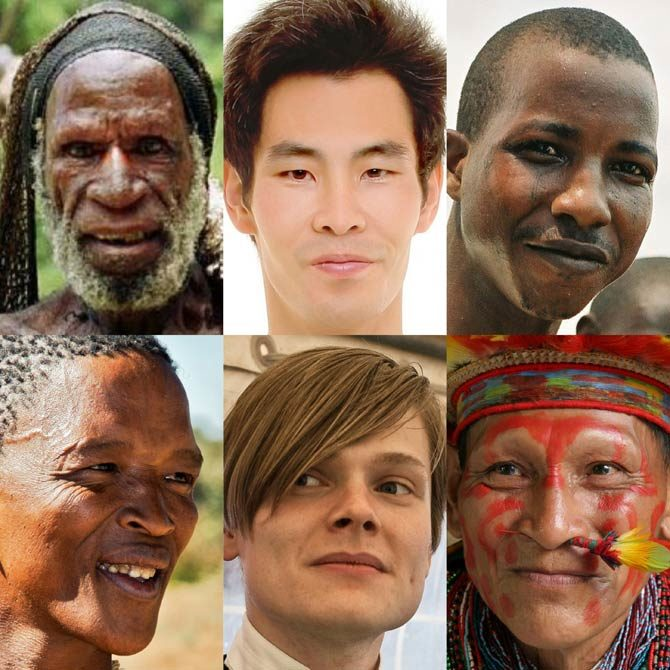
\includegraphics[width=.4\linewidth]{Homo sapiens.jpeg}
        \caption{Homo sapiens}
        \label{fig:Homo sapiens}
    \end{subfigure}
    \begin{subfigure}{.3\textwidth}
        \centering
        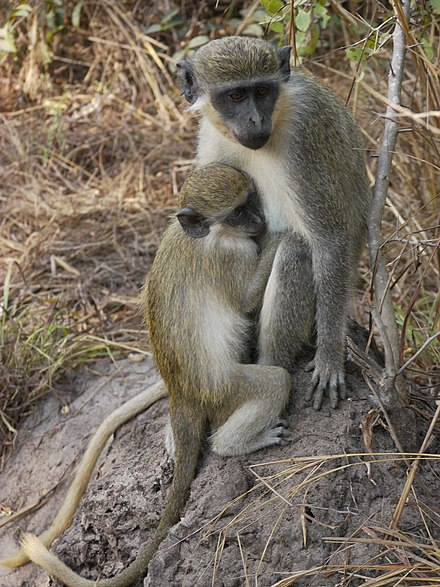
\includegraphics[width=.4\linewidth]{Chlorocebus sabaeus.jpeg}
        \caption{Chlorocebus sabaeus}
        \label{fig:Chlorocebus sabaeus}
    \end{subfigure}
    \begin{subfigure}{.3\textwidth}
        \centering
        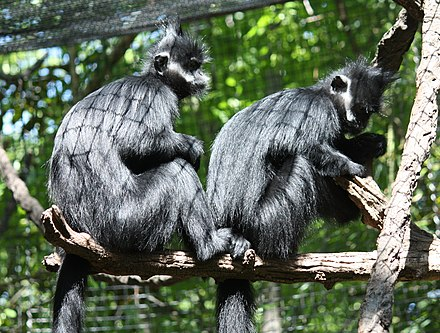
\includegraphics[width=.4\linewidth]{Trachypithecus francoisi.jpeg}
        \caption{Trachypithecus francoisi}
        \label{fig:Trachypithecus francoisi}
    \end{subfigure}
    \begin{subfigure}{.3\textwidth}
        \centering
        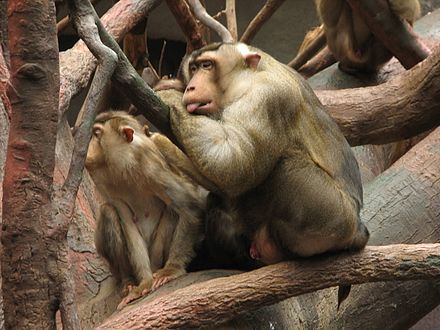
\includegraphics[width=.4\linewidth]{Macaca nemestrina.jpeg}
        \caption{Macaca nemestrina}
        \label{fig:Macaca nemestrina}
    \end{subfigure}
    \begin{subfigure}{.3\textwidth}
        \centering
        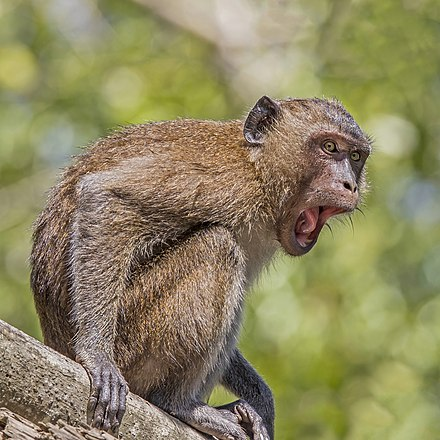
\includegraphics[width=.4\linewidth]{Macaca fascicularis.jpeg}
        \caption{Macaca fascicularis}
        \label{fig:Macaca fascicularis}
    \end{subfigure}
    \begin{subfigure}{.3\textwidth}
        \centering
        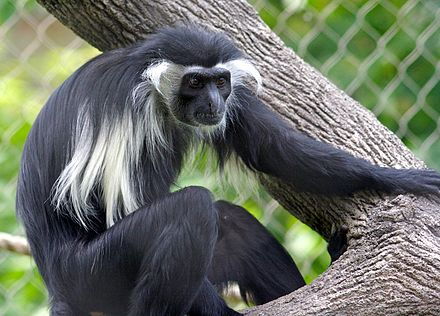
\includegraphics[width=.4\linewidth]{Colobus angolensis palliatus.jpeg}
        \caption{Colobus angolensis palliatus}
        \label{fig:Colobus angolensis palliatus}
    \end{subfigure}
    \begin{subfigure}{.3\textwidth}
        \centering
        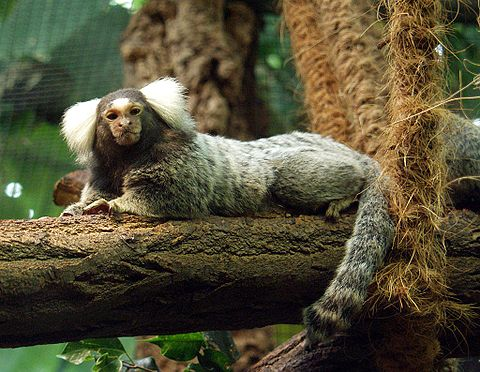
\includegraphics[width=.4\linewidth]{Callithrix jacchus.jpeg}
        \caption{Callithrix jacchus}
        \label{fig:Callithrix jacchus}
    \end{subfigure}
    \begin{subfigure}{.3\textwidth}
        \centering
        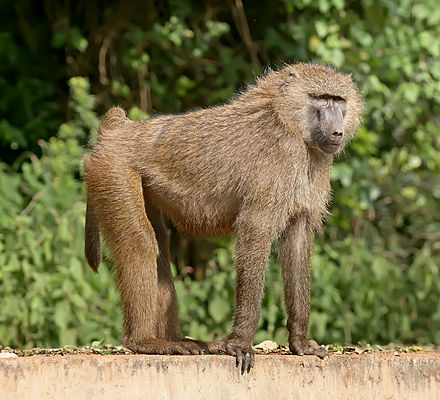
\includegraphics[width=.4\linewidth]{Papio anubis.jpeg}
        \caption{Papio anubis}
        \label{fig:Papio anubis}
    \end{subfigure}
\end{figure}


\section{Clustering}
\subsection{Clustering Method: k-medoids}
The situation is that we have 64 proteins and the 8*8 pair-wise distance matrix from local BlastP, but no metric space for the proteins, so we should use distance-matrix based clustering instead of metric-space based clustering (such as K-means). \\
Therefore, we choose the k-medoids clustering interface from Biopython Cluster library, which takes a distance matrix as the input. This clustering interface is designed for the k-medoids problem and implemented by the heuristic Partitioning Around Medoids (PAM) algorithm. \\
The \textbf{k-medoids problem} can be described as: \\
Given n points, integer k and similarity matrix D, to split the points into k clusters, \\
To minimize the distance between points labeled to be in a cluster and a point designated as the center of that cluster (medoid). \\
\\
This is a \textbf{NP-hard problem}, and usually solved approximatedly by \textbf{Partitioning Around Medoids (PAM)}: \\
1. (BUILD) Initialize: greedily select k of the n data points as the medoids to minimize the cost. \\
2. Associate each data point to the closest medoid. \\ 
3. (SWAP) While the cost of the configuration decreases: \\ 
For each medoid m, and for each non-medoid data point o:
Consider the swap of m and o, and compute the cost change. \\
If the cost change is the current best, remember this m and o combination. \\
Perform the best swap of m\_best and o\_best, if it decreases the cost function. Otherwise, the algorithm terminates.\\
\\
The k-medoids clustering interface provides a parameter "npass" to repeatly cluster the points using different initialzating medoids, and returns the best (by the least within-cluster sum of distances) clustering result. The larger the npass parameter is, the better and more stable the clustering result will be.\\

\subsection{Distance Matrix Definition}
We use the local BLASTP CommandLine to calculate the pair-wise BIT-scores from the 64 proteins. \\
We leave the parameters as default except for "max\_target\_seqs" which is set to 64 so that we will not omit the possibly similar pairs between different groups. \\
The commandline is: \\
"/usr/local/ncbi/blast/bin/blastp -subject 64\_samples.fasta -query 64\_samples.fasta -out test0.out -outfmt 10  -max\_target\_seqs 64" \\
This commandline gives a CSV file as the output, and the last column of the CSV file is the BLAST bit scores. \\
The result CSV file "test0.out" has 867 rows, which are the non-zero elements of the 64*64 bit score matrix. The matrix is quite sparse because the proteins from different groups are quite different from each other. \\
The BLAST bit score is an important measure that gives an indication about the statistical significance of an alignment. In simple terms, the higher the bit score, the more similar the two sequences are. \\
We normalize the bit score matrix by dividing each line by the diagnal elements, which means that we set the silimarity between a protein and itself to 1, so the terms of similarity matrix is between 0 and 1. \\
Considering that we need a distance matrix instead of similarity matrix, we use 1 - similarity\_matrix as the distance matrix.

\subsection{Clustering Result}
The clustering result depends on the initialzating medoids: 
if we set initialzating medoids from the same downloading group, 
the clustering result clusters will probably the same as the similar protein groups.
However, if some of the initialzating medoids are from the same group, the result could be different. \\
That is why we need the parameter "npass" to get more stable result by repeating the clustering using different initializations.\\

\subsubsection*{Unstable Solutions (Npass=1)}
The result is not stable and the error could be big (>10) when the npass parameter is small: \\
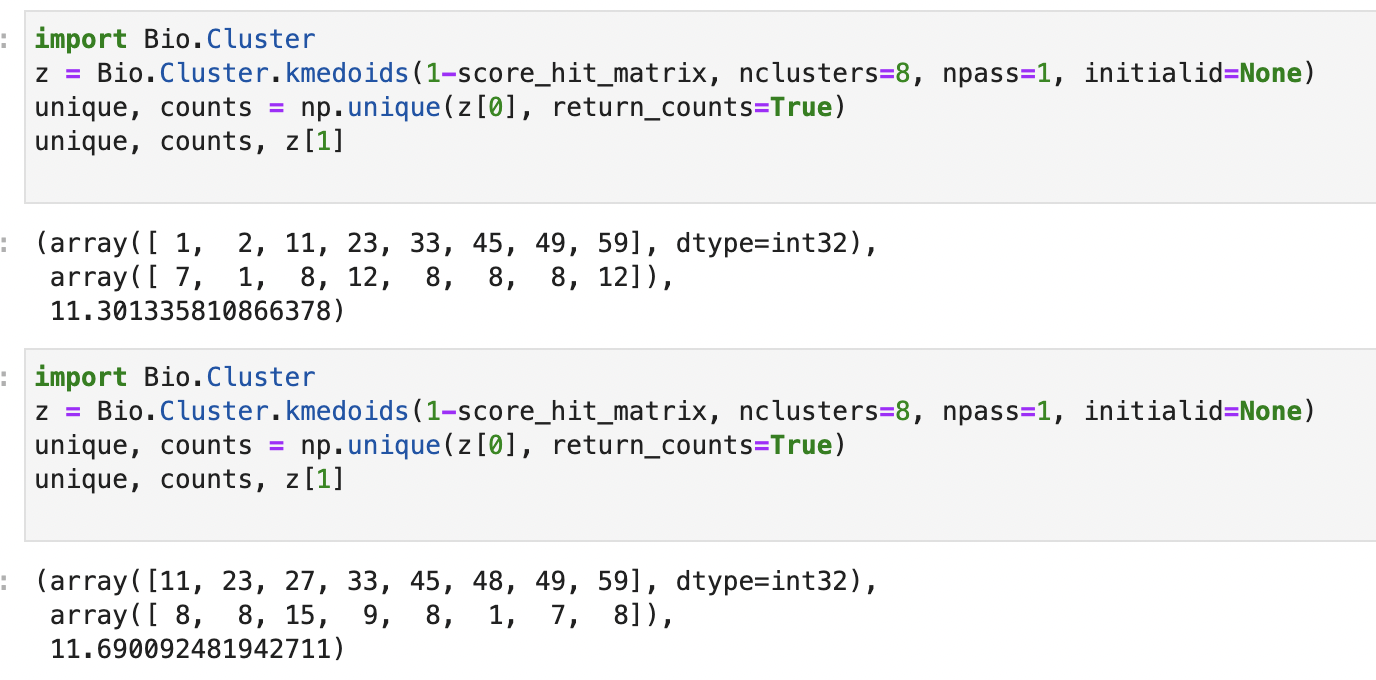
\includegraphics [width=.8\linewidth] {clustering_result_npass1.png} \\
\subsubsection*{Stable Optimal Solution (Npass=100)}
If we set a large "npass" parameter, the error is small (4.075), \\
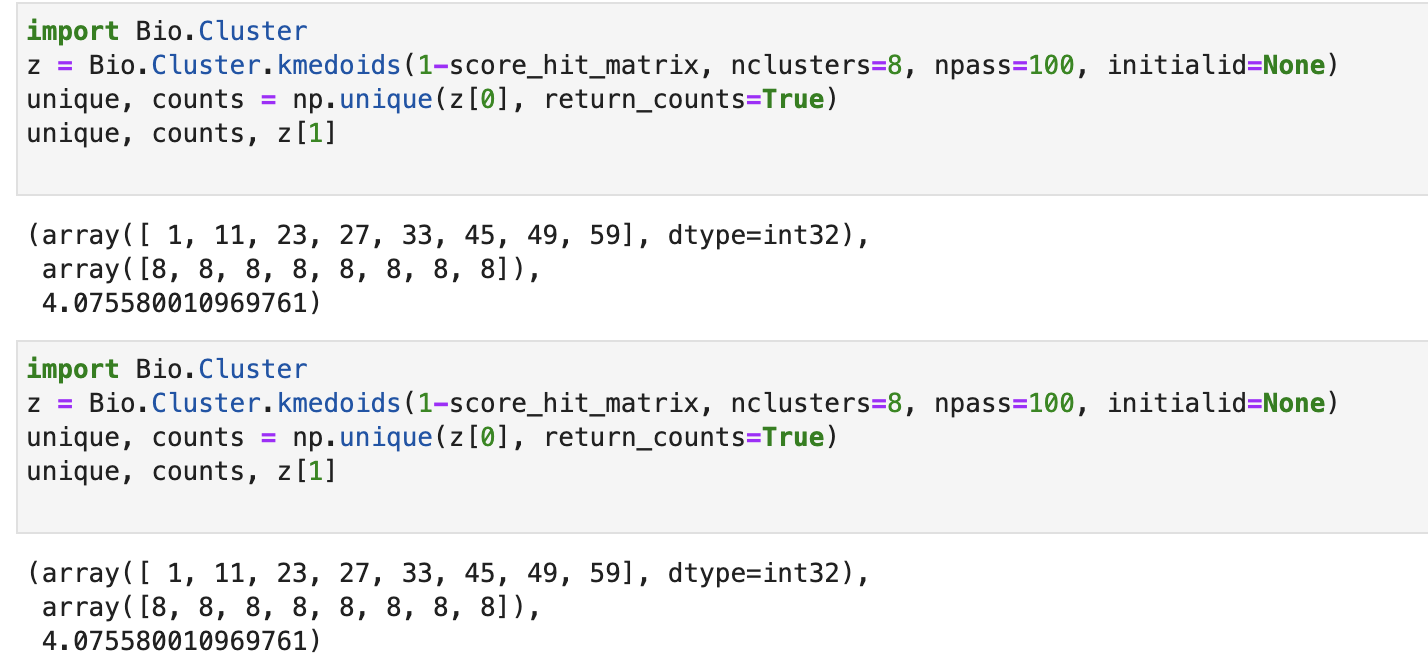
\includegraphics [width=.8\linewidth] {clustering_result_npass100.png} \\
and the result clusters are always exactly the same as the downloading similar protein groups, considering that the indices here are sorted by the downloading similar protein groups: 0-7 is the first group, ..., 56-63 is the last group.\\
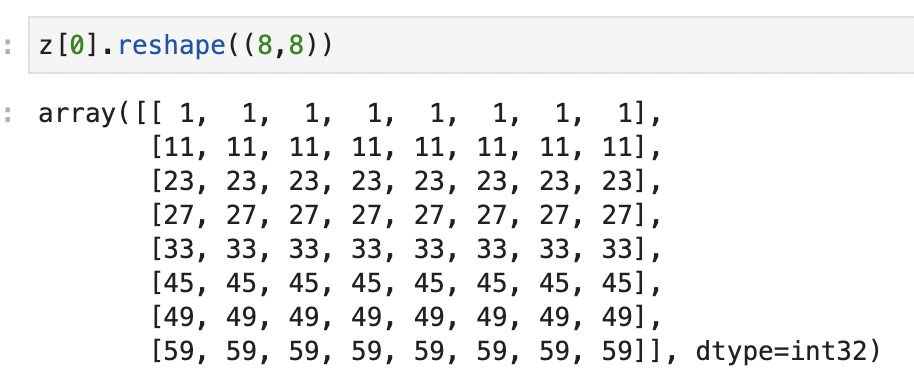
\includegraphics [width=.8\linewidth] {clusters.png} \\
although the 8 selected medoids are not from the same organism:\\
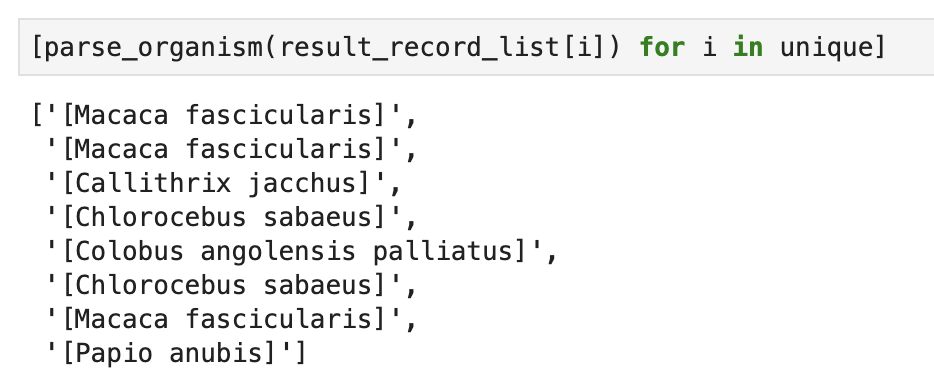
\includegraphics [width=.8\linewidth] {medoids.png} \\

\section{Phylogenetics}
A phylogenetic tree, also known as a phylogeny, is a diagram that depicts the lines of evolutionary descent of different species, organisms, or genes from a common ancestor.\\
We construct the phylogenetic tree of organisms inside each seperate group based on blast downloading similar proteins and k-medoids clusters.
\subsection{Method: UPGMA Algorithm}
UPGMA (unweighted pair group method with arithmetic mean) is a simple agglomerative (bottom-up) hierarchical clustering method. \\
The UPGMA algorithm constructs a rooted tree that reflects the structure present in a pairwise distance matrix. At each step, 
the nearest two clusters are combined into a higher-level cluster.  \\
The distance between any two clusters A and B, each of size |A| and |B|, 
is taken to be the average of all distances d(x, y) between pairs of objects $x \in A$ and $y \in B$, 
that is, the mean distance between elements of each cluster:\\
\begin{equation}
    d_{A,B}= \dfrac{1}{|A||B|} \sum_{i \in A, j\in B} {d_{i,j}}
\end{equation}
In other words, at each clustering step, the updated distance between the joined clusters $ A \cup B $ and a new cluster X is given by the proportional averaging of the $d_{A,X}$ and $d_{B,X}$ distances: \\
\begin{equation}
    d_{(A\cup B), X}= \dfrac{|A|\cdot d_{A,X}+ |B|\cdot d_{B,X} }{|A|+|B|}
\end{equation}
It is necessary to assume that all sequences evolve at the same rate by the theory of the Molecular Clock.

\subsection{Result of Building Trees}
\subsubsection{Examples of Separate trees for each "group" of proteins}
In each group there is only one protein for each organism, so we can denote the protein by the orgarnism name.\\
\begin{figure}[H]
    \centering
    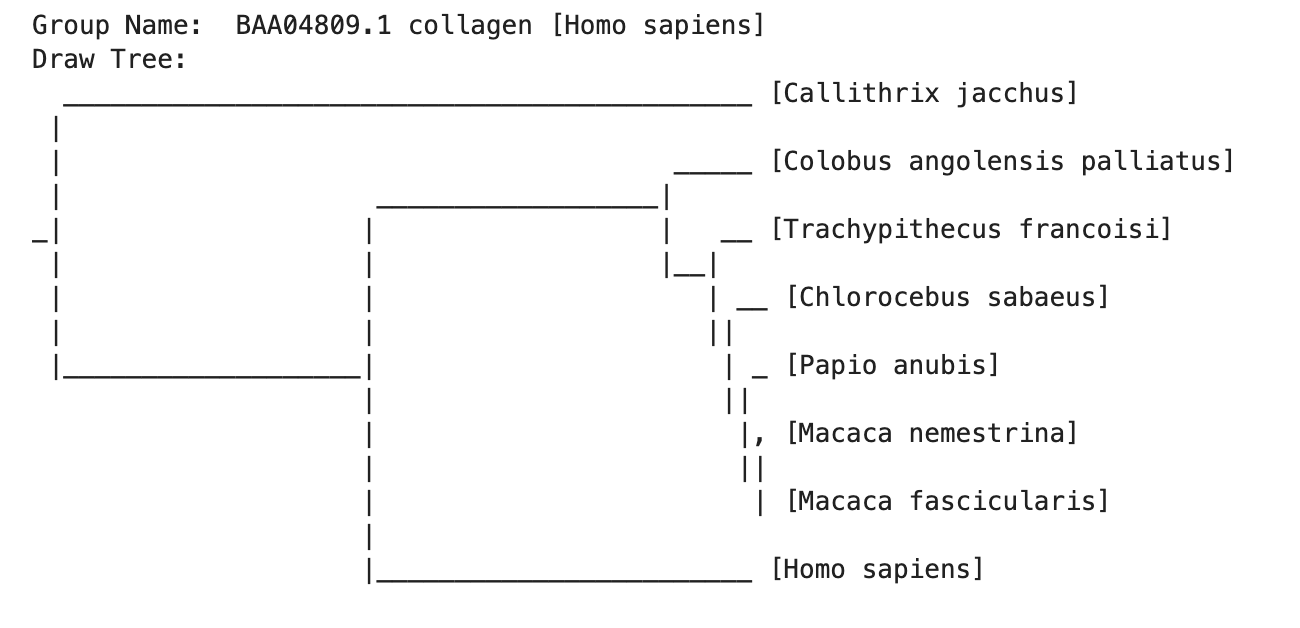
\includegraphics[width=.8\linewidth]{tree_group0.png}
    \caption{tree group 1 and also stable optimal cluster 1}
    \label{fig:tree_group0.png}
\end{figure}
\begin{figure}[H]
    \centering
    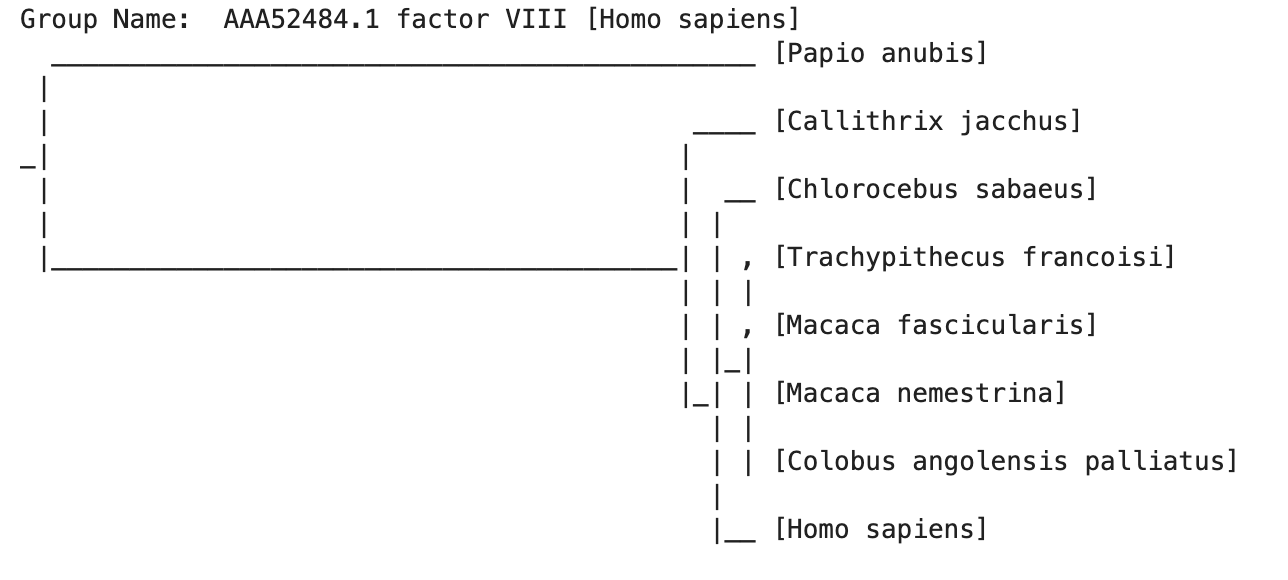
\includegraphics[width=.8\linewidth]{tree_group1.png}
    \caption{tree group 2 and also stable optimal cluster 2}
    \label{fig:tree_group1.png}
\end{figure}   

\subsubsection{Examples of Separate trees for clusters of proteins}
The stable optimal clusters (npass=100) are the same as the "group"s of proteins, so we just show the unstable clusters (n=1) here. \\
In each group there could be more than one protein for each organism, so we need to mark the protein names .\\
\begin{figure}[H]
    \centering
    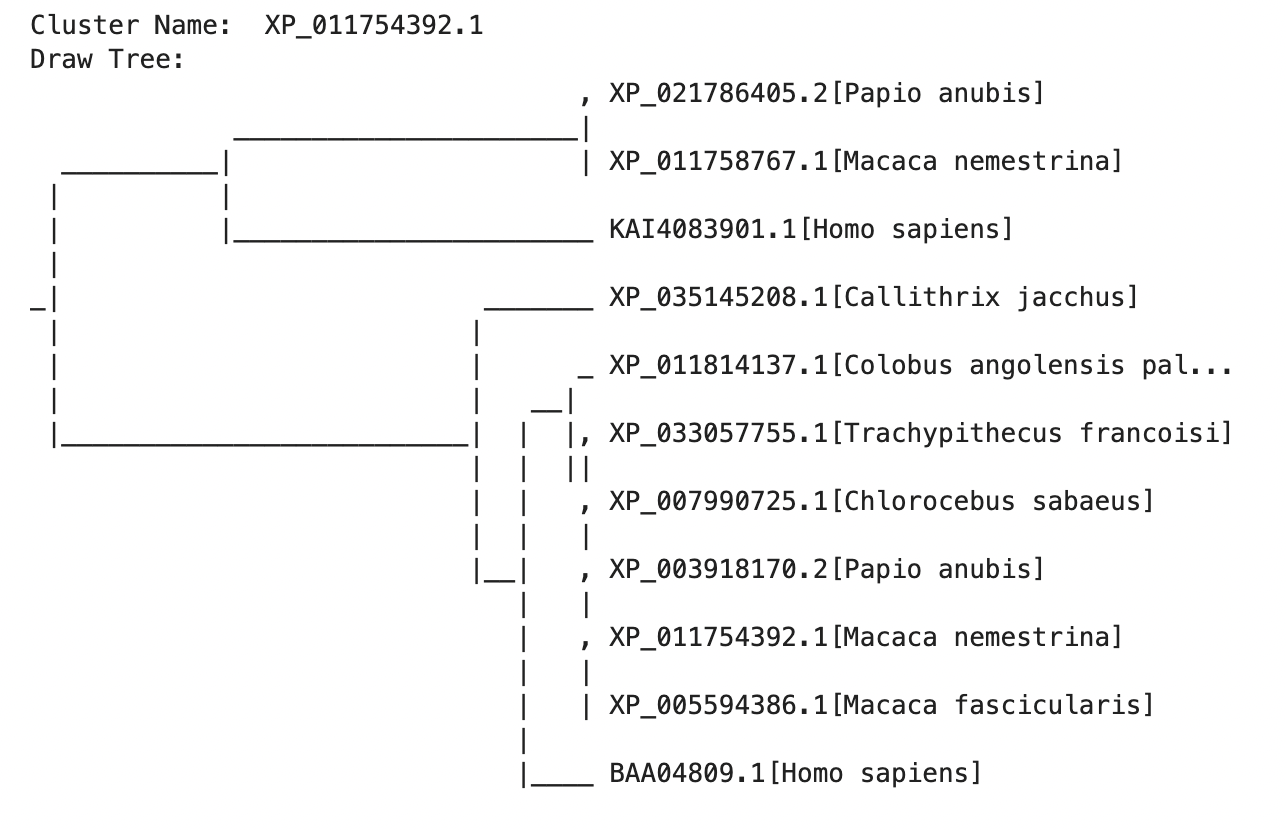
\includegraphics[width=.8\linewidth]{cluster_1.png}
    \caption{unstable cluster 1}
    \label{fig:cluster_1.png}
\end{figure}
\begin{figure}[H]
    \centering
    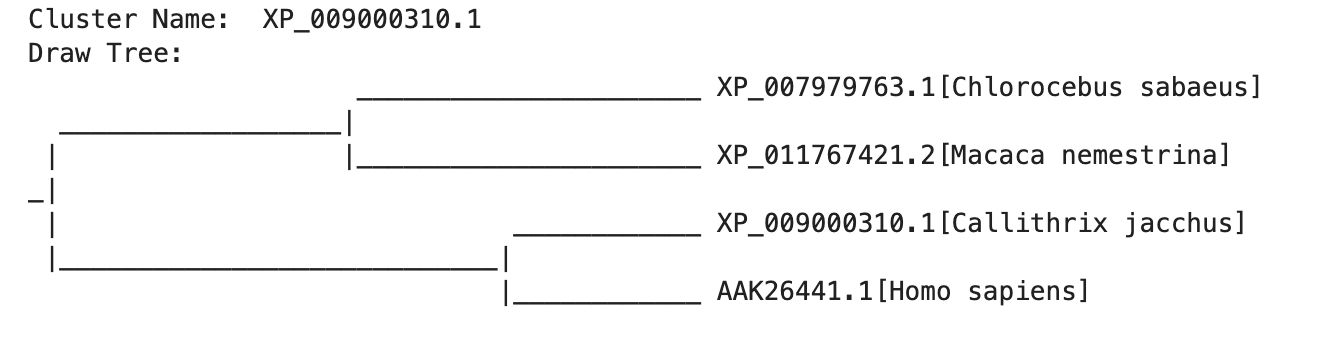
\includegraphics[width=.8\linewidth]{cluster_2.png}
    \caption{unstable cluster 2}
    \label{fig:cluster_2.png}
\end{figure}  


\subsubsection{One Common Tree for all proteins}

\begin{figure}[H]
    \centering
    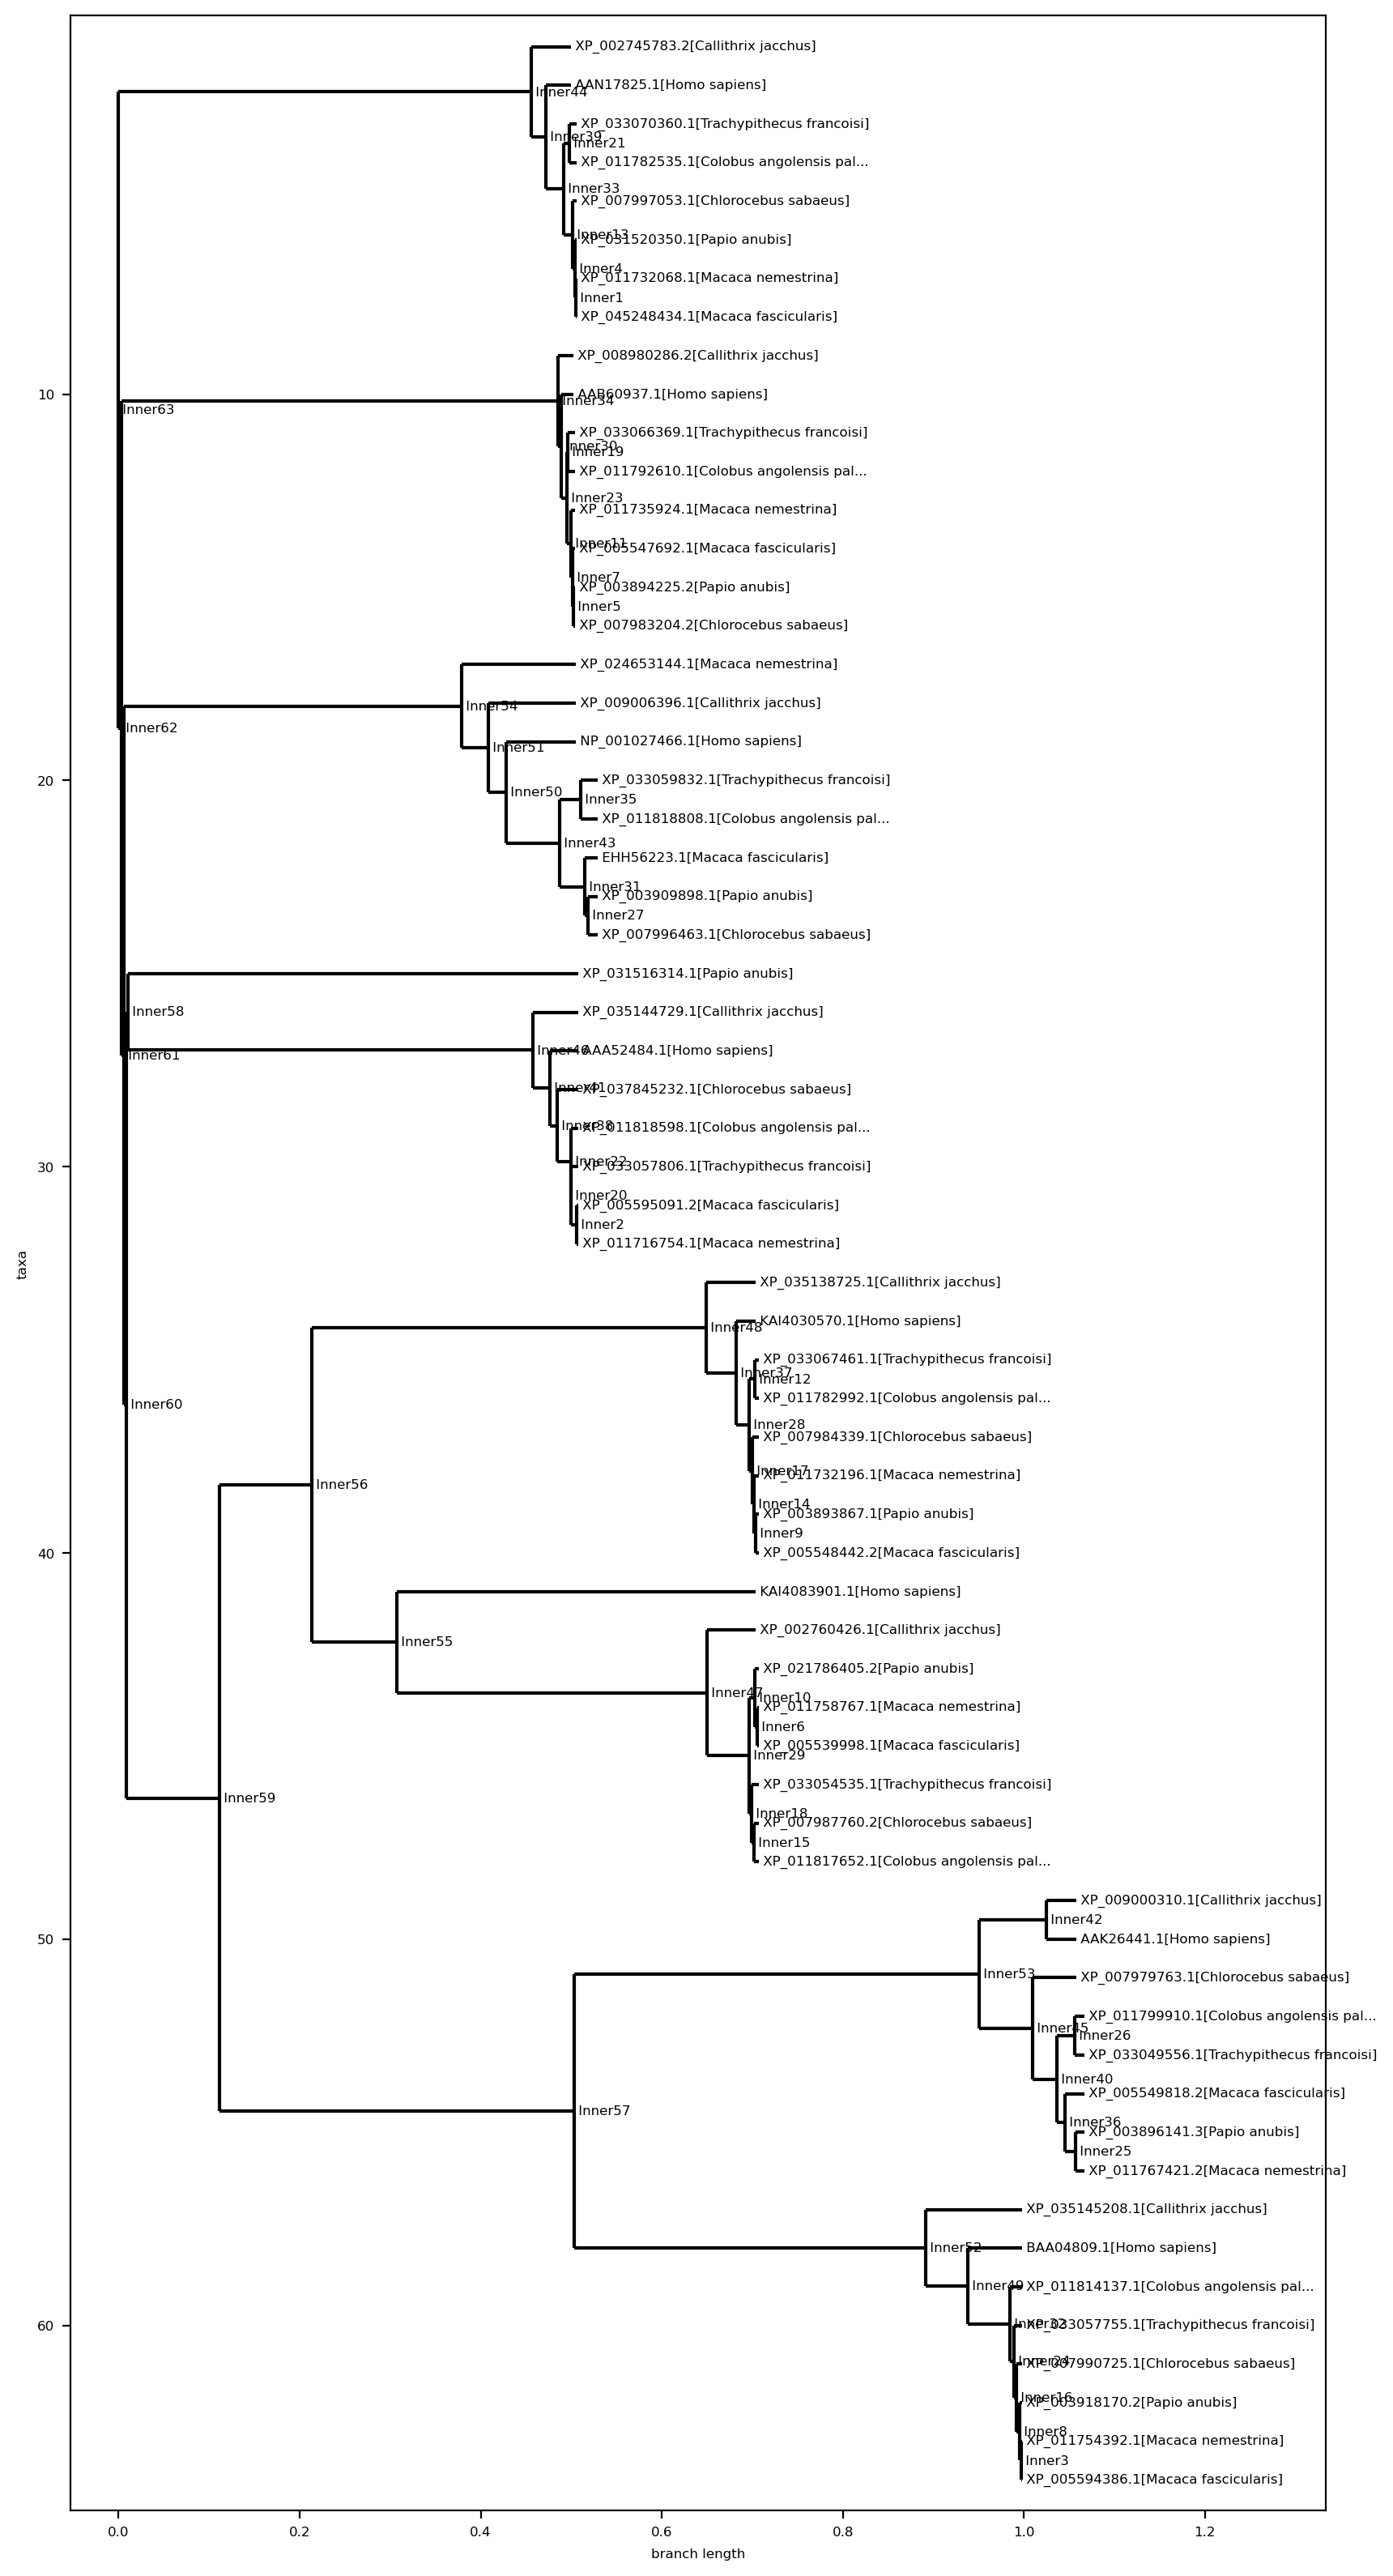
\includegraphics[width=.6\linewidth]{full_tree.png}
    \caption{full tree}
    \label{fig:full_tree.png}
\end{figure}  

\subsection{Consensus trees over organisms}
\subsubsection{Consensus tree over organisms From groups of proteins (and the stable optimal clusters)}
For a specific group of 8 proteins, we can let each protein represent its organism, and draw a phylogenetics tree for the 8 organisms. \\
Thus, we can calculate the consensus tree of 8 seperate trees, which means the most probable phylogenetics tree of the 8 organisms given such 8 groups of proteins.\\
Here, we use the majority consensus algorithm.\\
\begin{figure}[H]
    \centering
    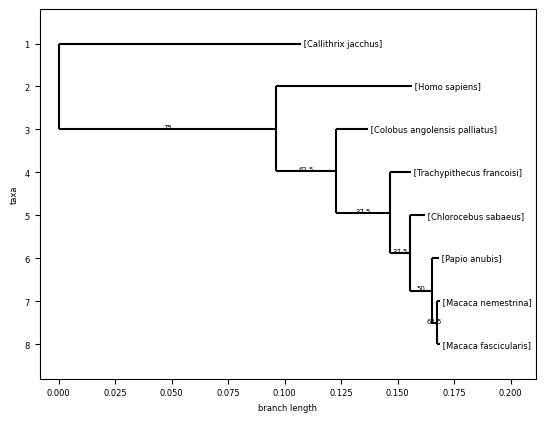
\includegraphics[width=.8\linewidth]{concensus_tree_of_groups.png}
    \caption{consensus tree of groups(or stable optimal clusters)}
    \label{fig:concensus_tree_of_groups.png}
\end{figure}  
According to the Consensus tree over organisms From groups of proteins (and the stable optimal clusters), we can conclude the probable Phylogenetics:\\
1. Callithrix jacchus is the remotest to other organisms, then is the homo sapiens, then is Colobus angolensis, ...  \\ 
2. Macaca fascicularis and Macaca nemestrina are the most similar organisms, which is implicated by their names. \\

\subsubsection{Consensus tree over organisms From unstable clusters is typically meanlingless}
The consensus phylogenetics tree is base on the consumption that each organism appears at most once in each group or cluster. \\
It is no problem for the original protein groups and the stable optimal clusters(which are the same as the original groups). \\
However, it is nearly impossible for unstable clusters to have such 8*8 result. \\
The existance of unstable clusters is because the bad initializating medoids (multiple medoids from the same original group).\\
Typically, there are always some unstable clusters whose size are not 8 because of the wrongly splitting of an orignal group, \\
but it could hardly happen that all the sizes are 8 but only some of the proteins are wrongly swapped among clusters. \\
Since we have some of the clusters with more than 8 elements, we cannot denote the tree leaves by organisms (Multiple leaves could share the same organism), \\
thus, the consensus tree of this case is meaningless.

\begin{figure}[H]
    \centering
    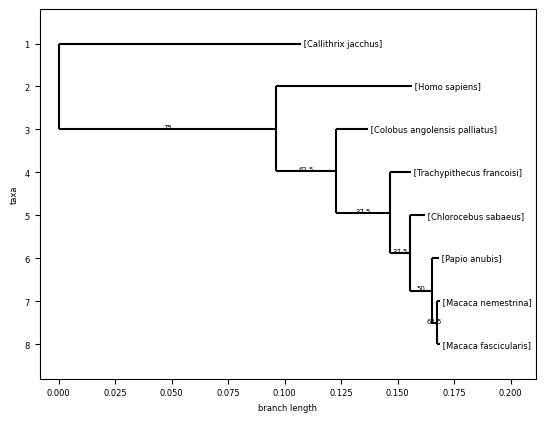
\includegraphics[width=.8\linewidth]{concensus_tree_of_groups.png}
    \caption{consensus tree of groups(or stable optimal clusters)}
    \label{fig:concensus_tree_of_groups.png}
\end{figure}  

% \subsection{Consensus trees over proteins}
% We can calculate a Consensus tree over all the proteins from the full tree 


\subsection{Colored visualizations}
\subsubsection{Implementation}
We can modify colors by setting the corresponding tree Clades, which can be calculated by Tree.get\_path.

\subsubsection{Colored by Groups}
\begin{figure}[H]
    \centering
    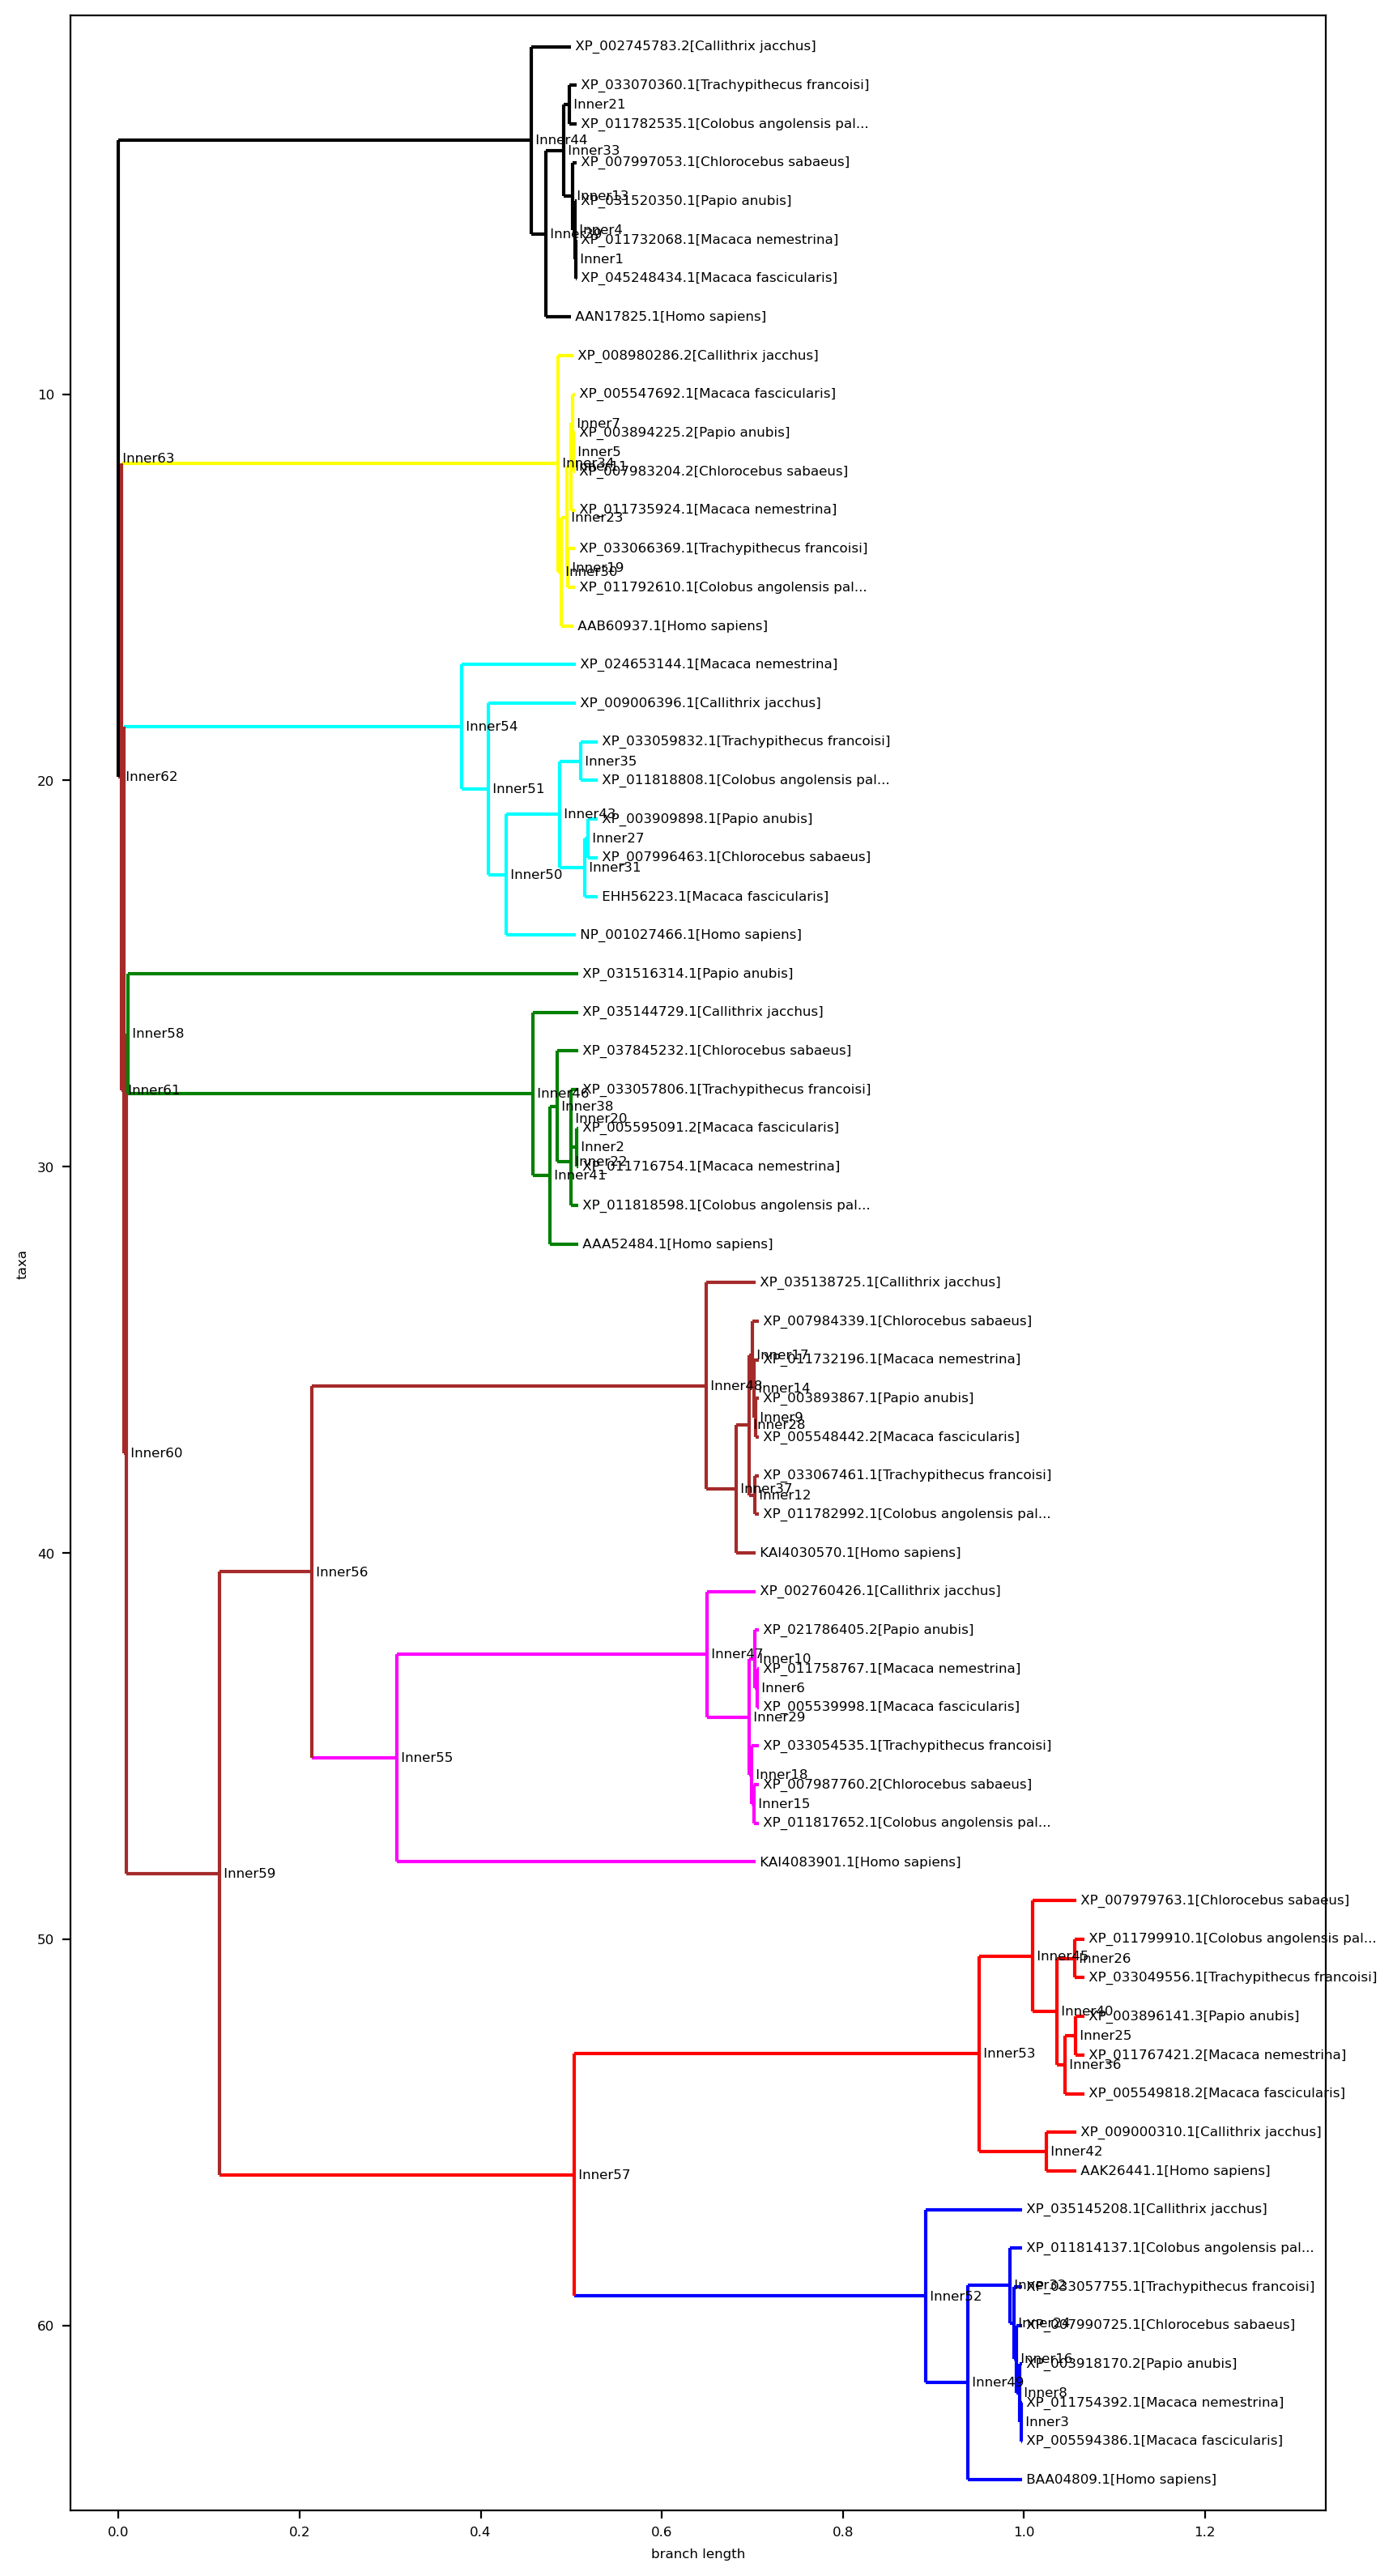
\includegraphics[width=.6\linewidth]{colored_group.png}
    \caption{colored by group}
    \label{fig:colored_group}
\end{figure}  
\subsubsection{Colored by Organisms}
\begin{figure}[H]
    \centering
    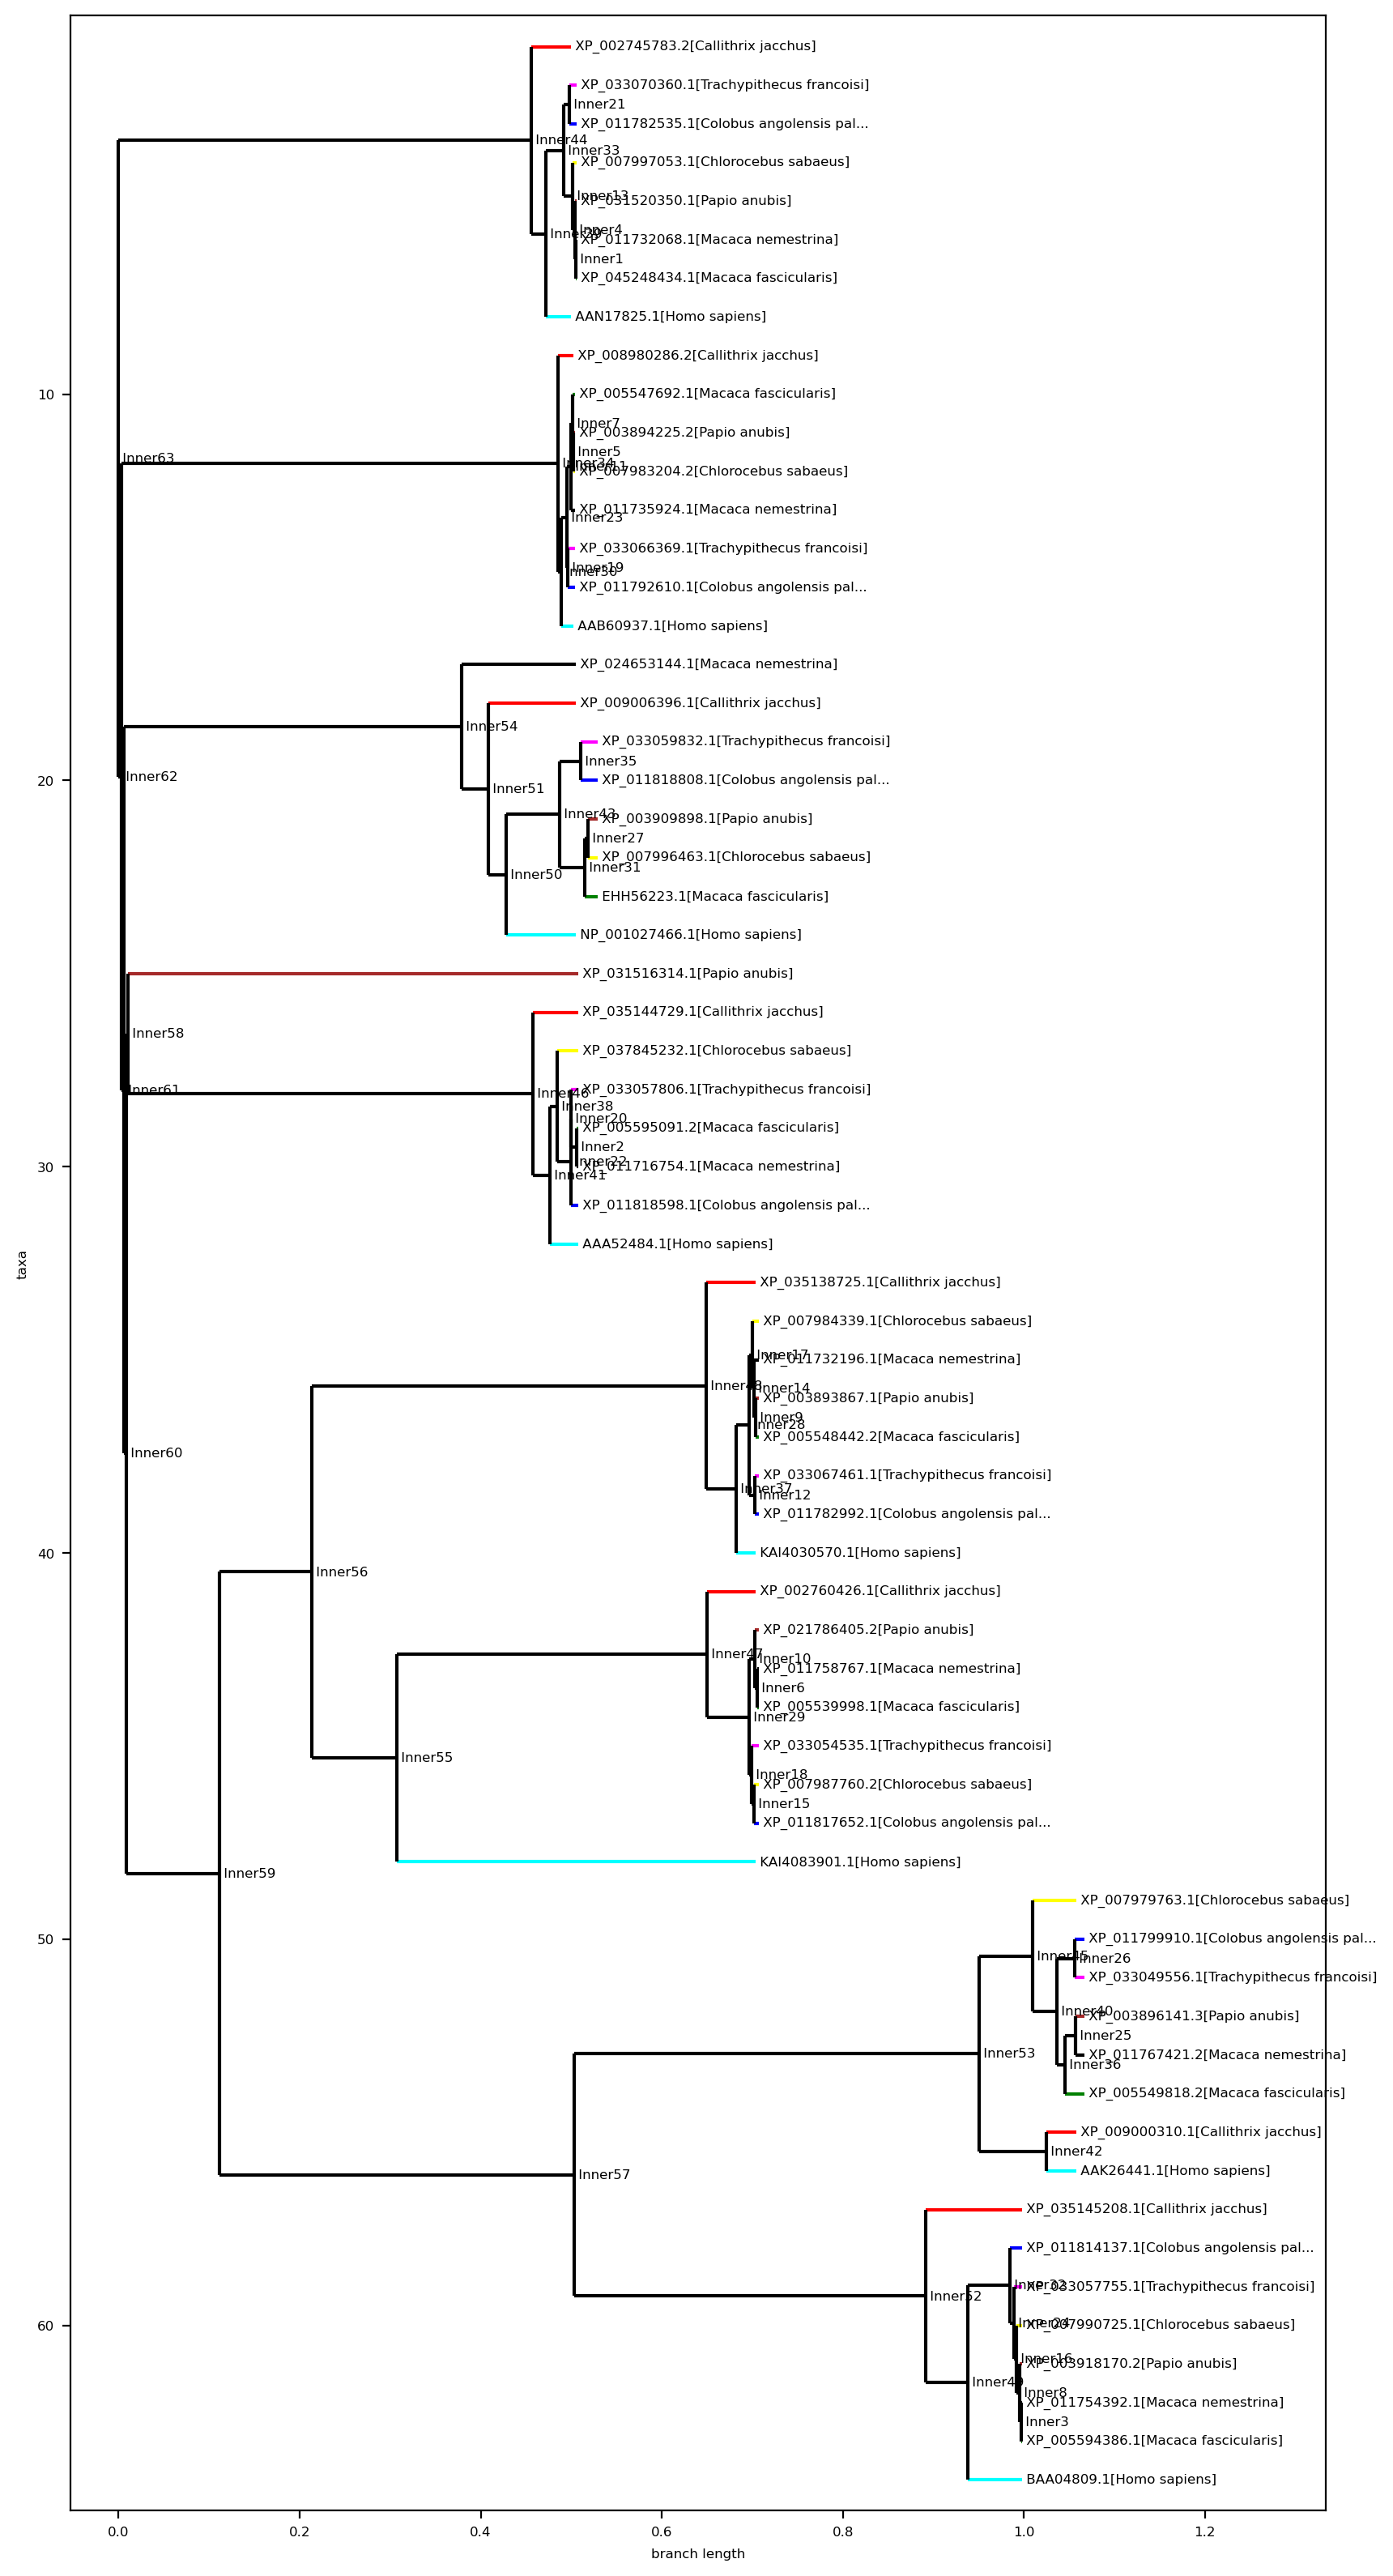
\includegraphics[width=.6\linewidth]{colored_organism.png}
    \caption{colored by organism}
    \label{fig:colored_organism}
\end{figure}

\section{Conclusions and Answers to the questions}
\subsection{Conclusions From the project}
According to the Consensus tree over organisms From groups of proteins (and the stable optimal clusters), we can conclude the probable Phylogenetics:\\
1. Callithrix jacchus is the remotest to other organisms, then is the homo sapiens, then is Colobus angolensis, ...  \\ 
2. Macaca fascicularis and Macaca nemestrina are the most similar organisms, which is implicated by their names. \\

In conclusion, we can use clustering  for multiple groups of similar proteins from the target organism groups, and get Phylogenetics trees to get the most probable evolution path over these organisms.

\subsection{Answers to the questions}
\subsubsection*{Question 2.f}
Q: What’s your observation? Which approach seems to work best? (The clusters vs the groups of proteins downloaded together)\\
\\
A: The two approaches here give the same reasonable Phylogenetics result for the 8 organisms. \\
In this dataset, the (stable optimal) clusters are totally the same as the groups of proteins downloaded together, so there is no differences here. \\
In my opinion, the clustering method (with large npass parameter to get the stable optimal result) could be better if we had very similar proteins in different groups of proteins.

\subsubsection*{Question 2.g}
Q: Are the trees similar to each other? Does the evolution look exactly the same in different
trees? \\
\\
A: The organism Phylogenetics trees of different groups/clusters are similar but not exactly the same. \\
Here the tree from group1/cluster1(collagen proteins) is not the same as the tree from group2/cluster2(factor VIII). \\
The tree in group1/cluster1(collagen proteins) is more similar to the consensus tree (actually the same). \\
Therefore, the evolution looks not the same in different groups of proteins.

\begin{figure}[H]
    \centering
    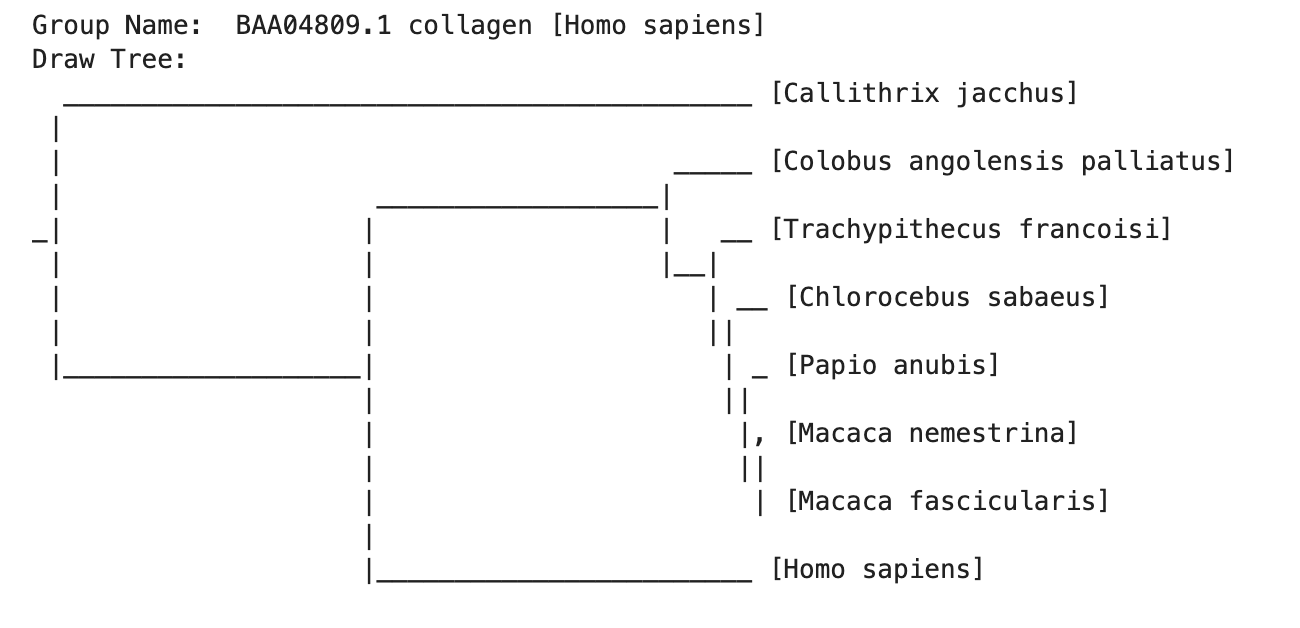
\includegraphics[width=.8\linewidth]{tree_group0.png}
    \caption{tree group 1 / cluster 1}
    \label{fig:tree_group11}
\end{figure}
\begin{figure}[H]
    \centering
    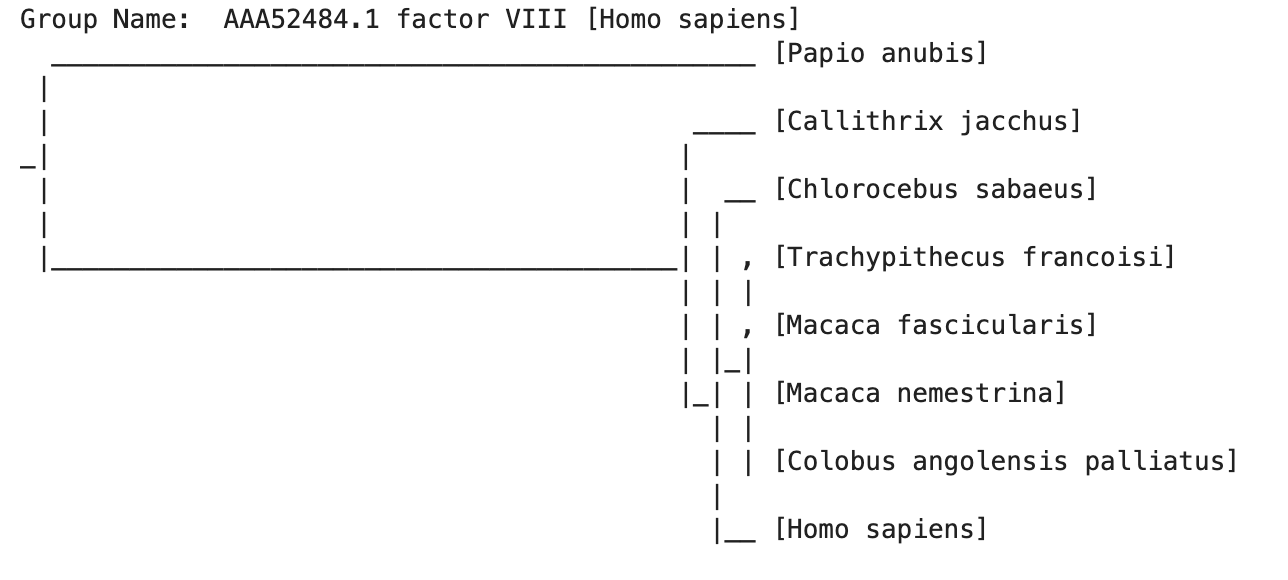
\includegraphics[width=.8\linewidth]{tree_group1.png}
    \caption{tree group 2 / cluster 2}
    \label{fig:tree_group21}
\end{figure}   
\begin{figure}[H]
    \centering
    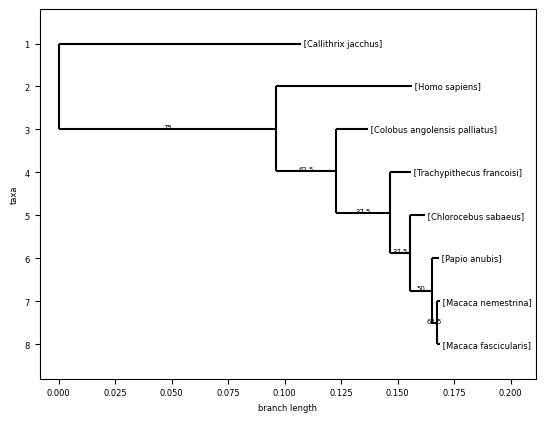
\includegraphics[width=.8\linewidth]{concensus_tree_of_groups.png}
    \caption{consensus tree of groups / clusters}
    \label{fig:concensus_tree.png}
\end{figure}  

\bibliography{refs}
\end{document}